% =====================================================================
% File        : user_defined_function_matlab.tex
% Deskripsi   : User-defined function di MATLAB: input, output,
%               beberapa input, dan beberapa output
% =====================================================================
\documentclass[aspectratio=169,11pt]{beamer}
\usetheme{metropolis}
\usepackage[utf8]{inputenc}
\usepackage{amsmath,amssymb}
\usepackage{booktabs}
\usepackage{listings}
\usepackage{tikz}
\usetikzlibrary{positioning,arrows.meta,shapes.misc,matrix}

\definecolor{kolom}{RGB}{31,119,180}
\definecolor{baris}{RGB}{214,39,40}
\definecolor{kode}{RGB}{245,245,245}

% Kotak "Masalah / Dicari" di awal slide contoh
\newcommand{\masalah}[3]{%
  \noindent\colorbox{kolom!8}{\parbox{\dimexpr\linewidth-2\fboxsep\relax}{%
    \footnotesize\textbf{Data:} #1\\[1pt]
    \textbf{Masalah:} #2\\[1pt]
    \textbf{Dicari:} #3}}\par\vspace{0.35em}}

\lstset{
  language=Matlab,
  basicstyle=\ttfamily\small,
  backgroundcolor=\color{kode},
  keywordstyle=\color{kolom}\bfseries,
  commentstyle=\color{gray}\itshape,
  frame=single, rulecolor=\color{gray!40},
  columns=fullflexible, keepspaces=true,
  xleftmargin=4pt, xrightmargin=4pt,
  showstringspaces=false
}

\title{User-Defined Function di MATLAB}
\subtitle{Input, output, beberapa input, dan beberapa output}
\author{Andreas Syaloom Kurniawan}
\institute{Faculty of Economics and Business, Universitas Gadjah Mada}
\date{}

\begin{document}

\maketitle

% ---------------------------------------------------------------------
\begin{frame}[fragile]{Anatomi sebuah function}
\begin{lstlisting}[basicstyle=\ttfamily\normalsize]
function [out1, out2, ...] = namaFungsi(in1, in2, ...)
    % badan fungsi: perhitungan
    out1 = ...;
    out2 = ...;
end
\end{lstlisting}
\vspace{0.3em}
\small
\begin{itemize}
  \item \texttt{function} \dots\ \texttt{end}: pembuka dan penutup definisi.
  \item \textcolor{baris}{\textbf{Output}} di kiri tanda \texttt{=}; lebih
        dari satu ditulis dalam kurung siku \texttt{[ ]}.
  \item \textcolor{kolom}{\textbf{Input}} di dalam kurung biasa \texttt{( )},
        dipisahkan koma.
  \item Setiap output \alert{wajib diberi nilai} di dalam badan fungsi.
\end{itemize}
\end{frame}

% ---------------------------------------------------------------------
\begin{frame}[fragile]{Di mana function disimpan?}
\begin{columns}[T]
\column{0.48\textwidth}
\textbf{1. File terpisah}
\begin{lstlisting}[basicstyle=\ttfamily\footnotesize]
% isi file: myfun1.m
function s = myfun1(x)
    ...
end
\end{lstlisting}
\small Nama file \alert{harus sama} dengan nama fungsi. File berada di
folder kerja (Current Folder) atau di \emph{path}.
\column{0.48\textwidth}
\textbf{2. Local function di dalam script}
\begin{lstlisting}[basicstyle=\ttfamily\footnotesize]
% isi file: latihan.m
a = myfun1(3);
disp(a)

function s = myfun1(x)
    ...
end
\end{lstlisting}
\small Definisi fungsi diletakkan di \alert{bagian paling bawah}
script (R2016b+). Hanya bisa dipanggil dari script itu.
\end{columns}
\end{frame}

% ---------------------------------------------------------------------
\begin{frame}[fragile]{Penamaan: nama file harus sama dengan nama function}
\begin{columns}[T]
\column{0.5\textwidth}
\small Function \texttt{myfun1} disimpan sebagai \alert{\texttt{myfun1.m}}.
\begin{itemize}\footnotesize
  \item \texttt{.m} = file \textbf{kode} (script atau function).
  \item \texttt{.mat} = file \textbf{data} (variabel hasil \texttt{save}),
        bukan kode.
\end{itemize}
\vspace{0.3em}
\small Jika nama tidak sama, MATLAB memakai \alert{nama file} dan mengabaikan
nama di baris \texttt{function}:
\begin{lstlisting}[basicstyle=\ttfamily\footnotesize]
% file: hitung.m
function s = myfun1(x)
    ...
end
\end{lstlisting}
\column{0.46\textwidth}
\begin{lstlisting}[basicstyle=\ttfamily\footnotesize, deletekeywords={function}]
>> hitung(3)    % jalan: nama file
>> myfun1(3)    % error
Unrecognized function or
variable 'myfun1'.
\end{lstlisting}
\small Editor MATLAB memberi \alert{peringatan kuning} untuk ketidakcocokan
ini. Tetap samakan namanya agar tidak membingungkan.
\end{columns}
\end{frame}

% ---------------------------------------------------------------------
\begin{frame}[fragile]{Aturan nama function (dan nama file)}
\begin{columns}[T]
\column{0.5\textwidth}
\small
\begin{enumerate}
  \item \textbf{Diawali huruf}, lalu huruf, angka, atau \texttt{\_}.
        Tidak boleh spasi atau \texttt{-}.
  \item \textbf{Jangan memakai nama fungsi bawaan}. Membuat \texttt{sum.m}
        atau \texttt{mean.m} sendiri akan \alert{menimpa} fungsi bawaan
        MATLAB.
  \item \textbf{File harus terlihat oleh MATLAB}: berada di Current Folder
        atau di path. Jika tidak, MATLAB tidak menemukannya walaupun namanya
        benar.
\end{enumerate}
\column{0.46\textwidth}
\footnotesize
\renewcommand{\arraystretch}{1.15}
\begin{tabular}{l l}
\toprule
Nama file & Status \\
\midrule
\texttt{myfun1.m} & valid \\
\texttt{hitung\_pdrb.m} & valid \\
\texttt{my-fun.m} & \textcolor{baris}{tidak valid} (\texttt{-}) \\
\texttt{2fun.m} & \textcolor{baris}{tidak valid} (diawali angka) \\
\texttt{sum.m} & \textcolor{baris}{berbahaya} (menimpa bawaan) \\
\bottomrule
\end{tabular}

\vspace{0.5em}
\small Cek sebuah nama sebelum dipakai:
\begin{lstlisting}[basicstyle=\ttfamily\scriptsize]
>> which sum
built-in (...\toolbox\matlab\datafun\sum)
>> which myfun1
'myfun1' not found.     % aman dipakai
\end{lstlisting}
\end{columns}
\end{frame}

% ---------------------------------------------------------------------
\begin{frame}[fragile]{Beberapa function dalam satu file: function utama dan local function}
\begin{columns}[T]
\column{0.55\textwidth}
\begin{lstlisting}[basicstyle=\ttfamily\scriptsize]
% file: myfun1.m
function s = myfun1(x)   % function utama
    y = bantu(x);
    s = log(y) - sqrt(y);
end

function y = bantu(x)    % local function
    y = x.^2 + 2*x - 4;
end
\end{lstlisting}
\begin{lstlisting}[basicstyle=\ttfamily\scriptsize, deletekeywords={function}]
>> myfun1(3)     % jalan
ans =
   -0.9187
>> bantu(3)      % error dari luar
Unrecognized function or variable 'bantu'.
\end{lstlisting}
\column{0.41\textwidth}
\footnotesize
\begin{itemize}
  \item Hanya function \alert{pertama} yang harus bernama sama dengan file.
        Function ini bisa dipanggil dari luar.
  \item Function berikutnya adalah \alert{local function}: namanya bebas,
        tetapi hanya bisa dipakai \textbf{di dalam file itu}.
  \item Hal yang sama berlaku untuk local function di bagian bawah
        \textbf{script}.
\end{itemize}
\vspace{0.3em}
\footnotesize Gunanya: memecah perhitungan panjang menjadi bagian kecil yang
rapi tanpa membuat banyak file.
\end{columns}
\end{frame}

% ---------------------------------------------------------------------
\begin{frame}[fragile]{Contoh 1: satu input, satu output}
\begin{columns}[T]
\column{0.54\textwidth}
\begin{lstlisting}[basicstyle=\ttfamily\scriptsize]
function s = myfun1(x) % output s, input x
    y = x*x + 2*x - 4;
    z = log(y);
    s = z - sqrt(y);
end
\end{lstlisting}
\small
Secara matematis:
\[
y = x^2 + 2x - 4,\quad z = \ln y,\quad s = z - \sqrt{y}
\]
\column{0.42\textwidth}
\begin{lstlisting}[basicstyle=\ttfamily\footnotesize]
>> myfun1(3)
ans =
   -0.9187
>> a = myfun1(3);  % disimpan
\end{lstlisting}
\small Cek manual untuk $x=3$:
\[
\begin{aligned}
y &= 9 + 6 - 4 = 11\\
z &= \ln 11 = 2.3979\\
s &= 2.3979 - 3.3166 = -0.9187
\end{aligned}
\]
\end{columns}
\end{frame}

% ---------------------------------------------------------------------
\begin{frame}[fragile]{Variabel di dalam function bersifat lokal}
\begin{columns}[c]
\column{0.5\textwidth}
\centering
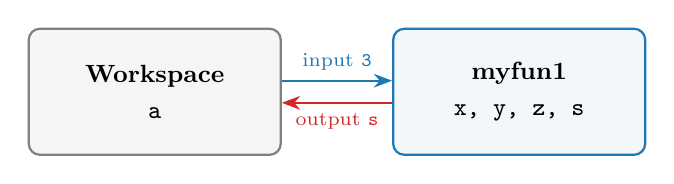
\begin{tikzpicture}[
  box/.style={draw, rounded corners, thick, minimum width=3.2cm,
              minimum height=1.6cm, align=center, font=\small},
  >=Stealth]
  \node[box, draw=gray, fill=gray!8] (ws) {\textbf{Workspace}\\[2pt]
        \texttt{a}};
  \node[box, draw=kolom, fill=kolom!6, right=1.4cm of ws] (fn)
        {\textbf{myfun1}\\[2pt]\texttt{x, y, z, s}};
  \draw[->, thick, kolom] ([yshift=4pt]ws.east) -- node[above, font=\scriptsize]
        {input \texttt{3}} ([yshift=4pt]fn.west);
  \draw[->, thick, baris] ([yshift=-4pt]fn.west) -- node[below, font=\scriptsize]
        {output \texttt{s}} ([yshift=-4pt]ws.east);
\end{tikzpicture}

\vspace{0.6em}
\small Hanya nilai \textbf{output} yang kembali ke workspace.
\column{0.46\textwidth}
\begin{lstlisting}[basicstyle=\ttfamily\footnotesize, deletekeywords={function}]
>> a = myfun1(3);
>> y
Unrecognized function or
variable 'y'.
\end{lstlisting}
\small \texttt{y} dan \texttt{z} hanya hidup selama fungsi berjalan, lalu
hilang. Nama \texttt{s} di dalam fungsi juga tidak harus sama dengan nama
variabel penampung (\texttt{a}).
\end{columns}
\end{frame}

% ---------------------------------------------------------------------
\begin{frame}[fragile]{Contoh 2: satu input, beberapa output}
\begin{columns}[T]
\column{0.5\textwidth}
\begin{lstlisting}[basicstyle=\ttfamily\footnotesize]
function [s, y, z] = myfun2(x)
    y = x*x + 2*x - 4;
    z = log(y);
    s = z - sqrt(y);
end
\end{lstlisting}
\small Perhitungannya sama dengan \texttt{myfun1}, tetapi \texttt{y} dan
\texttt{z} sekarang \alert{ikut dikembalikan} sebagai output.
\column{0.46\textwidth}
\begin{lstlisting}[basicstyle=\ttfamily\footnotesize]
>> [s, y, z] = myfun2(3)
s =
   -0.9187
y =
    11
z =
    2.3979
\end{lstlisting}
\end{columns}
\end{frame}

% ---------------------------------------------------------------------
\begin{frame}[fragile]{Mengambil sebagian output}
\begin{columns}[T]
\column{0.5\textwidth}
\begin{lstlisting}[basicstyle=\ttfamily\footnotesize]
>> s = myfun2(3)       % output ke-1
s =
   -0.9187
>> [s, y] = myfun2(3)  % ke-1 dan ke-2
>> [~, y] = myfun2(3)  % lewati s
y =
    11
>> [~, ~, z] = myfun2(3)
z =
    2.3979
\end{lstlisting}
\column{0.46\textwidth}
\small
\begin{itemize}
  \item Output diambil \alert{berurutan dari kiri}, sesuai urutan di
        \texttt{[s, y, z]}.
  \item Tanda \texttt{\textasciitilde} membuang output yang tidak dibutuhkan.
  \item Yang menentukan urutan adalah \textbf{posisi}, bukan nama:
        \texttt{[a, b] = myfun2(3)} memberi \texttt{a = s} dan
        \texttt{b = y}.
\end{itemize}
\end{columns}
\end{frame}

% ---------------------------------------------------------------------
\begin{frame}[fragile]{Contoh 3: beberapa input, satu output}
\begin{columns}[T]
\column{0.6\textwidth}
\begin{lstlisting}[basicstyle=\ttfamily\scriptsize]
function mu = myfun3(s, t)   % output mu, input s dan t
    nilai = s.^2 + 2*t - log(10);
    mu = exp(nilai);
end
\end{lstlisting}
\small Secara matematis:
\[
\mu = \exp\!\left(s^2 + 2t - \ln 10\right) = \frac{e^{s^2+2t}}{10}
\]
\column{0.36\textwidth}
\begin{lstlisting}[basicstyle=\ttfamily\footnotesize]
>> myfun3(1, 2)
ans =
   14.8413
>> myfun3(2, 1)  % urutan!
ans =
  40.3429
\end{lstlisting}
\small Input dicocokkan berdasarkan \alert{posisi}: argumen pertama
masuk ke \texttt{s}, argumen kedua ke \texttt{t}.
\end{columns}
\end{frame}

% ---------------------------------------------------------------------
\begin{frame}[fragile]{Operator titik: function yang menerima vektor}
\begin{columns}[T]
\column{0.5\textwidth}
\small \texttt{myfun3} memakai \texttt{s.\textasciicircum2} (per elemen), sehingga
bisa menerima vektor:
\begin{lstlisting}[basicstyle=\ttfamily\footnotesize]
>> myfun3([1 2], 2)
ans =
   14.8413  298.0958
\end{lstlisting}
\small \texttt{myfun1} memakai \texttt{x*x} (perkalian matriks):
\begin{lstlisting}[basicstyle=\ttfamily\footnotesize, deletekeywords={for}]
>> myfun1([1 2 3])
Error using  *
Incorrect dimensions for matrix
multiplication. ...
\end{lstlisting}
\column{0.46\textwidth}
\small
\textbf{Perbaikan}: ganti dengan operator per elemen.
\begin{lstlisting}[basicstyle=\ttfamily\footnotesize]
function s = myfun1v(x)
    y = x.^2 + 2*x - 4;
    z = log(y);
    s = z - sqrt(y);
end
\end{lstlisting}
\small \texttt{log}, \texttt{sqrt}, dan \texttt{exp} sudah bekerja per
elemen; yang perlu diperhatikan hanya \texttt{*}, \texttt{/}, dan
\texttt{\textasciicircum}.
\end{columns}
\end{frame}

% ---------------------------------------------------------------------
\begin{frame}[fragile]{Hati-hati domain: \texttt{log} dan \texttt{sqrt}}
\begin{columns}[T]
\column{0.5\textwidth}
\small
\texttt{myfun1} hanya bernilai real jika $y > 0$:
\[
x^2 + 2x - 4 > 0
\]
\[
\Longleftrightarrow\;
x < -1-\sqrt5 \;\text{ atau }\; x > -1+\sqrt5
\]
yaitu $x < -3.236$ atau $x > 1.236$.

\vspace{0.4em}
Di luar itu MATLAB \alert{tidak error}, tetapi diam-diam mengembalikan
bilangan \textbf{kompleks}.
\column{0.46\textwidth}
\begin{lstlisting}[basicstyle=\ttfamily\footnotesize]
>> myfun1(0)       % y = -4
ans =
   1.3863 + 1.1416i
>> isreal(myfun1(0))
ans = 0
\end{lstlisting}
\small Bisa ditambahkan pengecekan di awal fungsi:
\begin{lstlisting}[basicstyle=\ttfamily\footnotesize]
if any(y <= 0)
    error('y harus > 0');
end
\end{lstlisting}
\end{columns}
\end{frame}

% ---------------------------------------------------------------------
\begin{frame}[fragile]{Alternatif singkat: anonymous function}
\begin{columns}[T]
\column{0.5\textwidth}
\small Untuk rumus satu baris, tidak perlu file terpisah:
\begin{lstlisting}[basicstyle=\ttfamily\footnotesize]
>> f = @(s,t) exp(s.^2 + 2*t - log(10));
>> f(1, 2)
ans =
   14.8413
\end{lstlisting}
\small \texttt{f} di sini setara dengan \texttt{myfun3}.
\column{0.46\textwidth}
\small
\renewcommand{\arraystretch}{1.2}
\begin{tabular}{l l}
\toprule
\texttt{function} & anonymous \texttt{@} \\
\midrule
banyak baris & satu ekspresi \\
banyak output & satu output \\
file / bagian bawah script & di mana saja \\
\bottomrule
\end{tabular}
\end{columns}
\end{frame}

% ---------------------------------------------------------------------
\begin{frame}{Ringkasan}
\centering\small
\renewcommand{\arraystretch}{1.3}
\begin{tabular}{l l l}
\toprule
Pola & Definisi & Pemanggilan \\
\midrule
1 input, 1 output & \texttt{function s = myfun1(x)} & \texttt{a = myfun1(3)} \\
1 input, banyak output & \texttt{function [s,y,z] = myfun2(x)} & \texttt{[s,y,z] = myfun2(3)} \\
banyak input, 1 output & \texttt{function mu = myfun3(s,t)} & \texttt{mu = myfun3(1,2)} \\
lewati output & --- & \texttt{[\textasciitilde,y] = myfun2(3)} \\
\bottomrule
\end{tabular}

\vspace{0.8em}
\raggedright
\begin{itemize}
  \item Input dan output dicocokkan berdasarkan \alert{posisi}.
  \item Variabel di dalam fungsi bersifat lokal.
  \item Gunakan \texttt{.*}, \texttt{./}, \texttt{.\textasciicircum} agar fungsi
        menerima vektor.
\end{itemize}
\end{frame}

% =====================================================================
\section{Handling Complex Input}
% =====================================================================

\begin{frame}{Input tidak selamanya berupa satu angka}
\small
Sejauh ini \texttt{myfun1}, \texttt{myfun2}, dan \texttt{myfun3} menerima
\textbf{satu angka}, misalnya \texttt{myfun1(3)}. Di pekerjaan nyata, input
sebuah fungsi sering datang dalam \alert{bentuk lain}:

\vspace{0.4em}
\footnotesize
\renewcommand{\arraystretch}{1.18}
\centering
\begin{tabular}{l l l}
\toprule
Bentuk input & Contoh di ekonomi & Wadah MATLAB \\
\midrule
Vektor & inflasi bulanan 2015--2024 (120 observasi) & array $120\times1$ \\
Matriks & PDRB 38 provinsi $\times$ 10 tahun & array $38\times10$ \\
\textbf{List} & harga beberapa komoditas, panjang data berbeda & cell array \\
Record & parameter model: $\beta$, $\sigma$, $\alpha$ & struct \\
Data tabular & hasil survei dari CSV/Excel & table \\
Teks & nama provinsi, nama file & string / char \\
Fungsi & rumus yang akan diintegralkan atau dioptimasi & function handle \texttt{@} \\
\bottomrule
\end{tabular}

\vspace{0.5em}
\raggedright\small
Section ini fokus pada dua bentuk yang paling sering muncul:
\alert{list (cell array)} dan \alert{matriks}.
\end{frame}

% ---------------------------------------------------------------------
\begin{frame}[fragile]{Tiga pertanyaan sebelum menulis function}
\begin{columns}[T]
\column{0.55\textwidth}
\small
\begin{enumerate}
  \item \textbf{Input-nya berbentuk apa?}\\
        Angka, vektor, matriks, cell, atau struct? Berapa ukurannya?
  \item \textbf{Output-nya ingin berbentuk apa?}\\
        Satu angka (ringkasan), array (satu nilai per item), atau matriks
        (beberapa nilai per item)?
  \item \textbf{Bagaimana cara ``berjalan'' di dalam input?}\\
        Loop per elemen/sel, argumen \texttt{dim}, atau operasi vektor?
\end{enumerate}
\vspace{0.3em}
\footnotesize Jawaban pertanyaan 2 menentukan cara \emph{preallocate};
jawaban pertanyaan 3 menentukan cara mengisi output.
\column{0.41\textwidth}
\small Cara memeriksa bentuk input:
\begin{lstlisting}[basicstyle=\ttfamily\scriptsize]
>> class(x)      % tipe: 'double', 'cell'
>> size(x)       % ukuran
>> numel(x)      % jumlah elemen/sel
>> iscell(x)     % cell?
>> isnumeric(x)  % angka?
\end{lstlisting}
\footnotesize Satu fungsi bisa memakai pengecekan ini untuk menolak input
yang salah bentuk:
\begin{lstlisting}[basicstyle=\ttfamily\scriptsize]
if ~iscell(c)
    error('Input harus cell array');
end
\end{lstlisting}
\end{columns}
\end{frame}

% ---------------------------------------------------------------------
\begin{frame}[fragile]{Data contoh (1): list \texttt{c}}
\begin{columns}[T]
\column{0.5\textwidth}
\small Kita buat list (cell array) berisi tiga sel:
\begin{lstlisting}[basicstyle=\ttfamily\footnotesize]
>> c = {[1 2 3], [4 5], 6}
c =
  1x3 cell array
    {[1 2 3]}    {[4 5]}    {[6]}
>> c{1}      % isi sel 1: [1 2 3]
>> c{2}      % isi sel 2: [4 5]
>> c{3}      % isi sel 3: 6
\end{lstlisting}
\footnotesize Kurung kurawal \texttt{c\{i\}} membuka isi sel ke-$i$.
\column{0.46\textwidth}
\centering
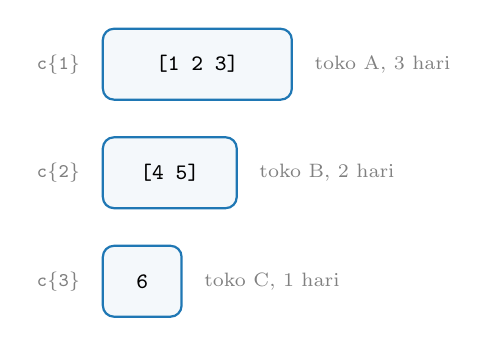
\begin{tikzpicture}[
  sel/.style={draw=kolom, thick, rounded corners, minimum height=0.9cm,
              font=\footnotesize\ttfamily, fill=kolom!5},
  lab/.style={font=\scriptsize, text=gray}]
  \node[sel, minimum width=2.4cm] (s1) {[1 2 3]};
  \node[sel, minimum width=1.7cm, below=0.45 of s1.south west, anchor=north west] (s2) {[4 5]};
  \node[sel, minimum width=1.0cm, below=0.45 of s2.south west, anchor=north west] (s3) {6};
  \node[lab, left=0.15 of s1] {\texttt{c\{1\}}};
  \node[lab, left=0.15 of s2] {\texttt{c\{2\}}};
  \node[lab, left=0.15 of s3] {\texttt{c\{3\}}};
  \node[lab, right=0.15 of s1, align=left] {toko A, 3 hari};
  \node[lab, right=0.15 of s2, align=left] {toko B, 2 hari};
  \node[lab, right=0.15 of s3, align=left] {toko C, 1 hari};
\end{tikzpicture}

\vspace{0.4em}
\raggedright\footnotesize
\begin{itemize}
  \item 3 sel dengan \alert{panjang berbeda}: $1\times3$, $1\times2$, $1\times1$.
  \item \texttt{numel(c)} = 3 sel; total angkanya 6.
  \item Karena panjangnya berbeda, data ini \alert{tidak bisa} disimpan
        sebagai satu matriks.
\end{itemize}
\end{columns}
\end{frame}

% ---------------------------------------------------------------------
\begin{frame}[fragile]{Data contoh (2): matriks \texttt{A}}
\begin{columns}[c]
\column{0.26\textwidth}
\begin{lstlisting}[basicstyle=\ttfamily\footnotesize]
>> A = magic(3)
A =
     8     1     6
     3     5     7
     4     9     2
\end{lstlisting}
\column{0.38\textwidth}
\centering
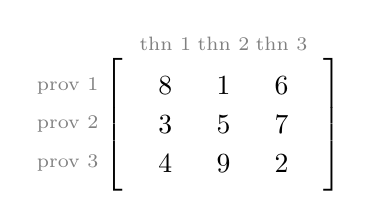
\begin{tikzpicture}
\matrix (m) [matrix of math nodes, nodes={minimum width=2.1em, minimum height=1.4em},
             left delimiter={[}, right delimiter={]}]
{ 8 & 1 & 6\\ 3 & 5 & 7\\ 4 & 9 & 2\\ };
\foreach \c in {1,2,3}
  \node[font=\scriptsize, text=gray] at ([yshift=8pt]m-1-\c.north) {thn \c};
\foreach \r in {1,2,3}
  \node[font=\scriptsize, text=gray, anchor=east] at ([xshift=-10pt]m-\r-1.west) {prov \r};
\end{tikzpicture}
\column{0.3\textwidth}
\small Cerita: \alert{baris = provinsi}, \alert{kolom = tahun}.

\vspace{0.3em}
Misalnya \texttt{A(2,3) = 7} adalah nilai provinsi 2 pada tahun 3.
\end{columns}

\vspace{0.8em}
\centering\footnotesize
\renewcommand{\arraystretch}{1.15}
\begin{tabular}{l c c c}
\toprule
Input $\backslash$ Output & angka & array & matriks \\
\midrule
list \texttt{c} & \texttt{totalList} & \texttt{jumlahPerItem} & \texttt{statPerItem} \\
matriks \texttt{A} & \texttt{rentang} & \texttt{maksPerBaris} & \texttt{standarkan} \\
\bottomrule
\end{tabular}

\vspace{0.3em}
\scriptsize Peta enam contoh berikut: setiap kombinasi bentuk input dan bentuk
output.
\end{frame}

% ---------------------------------------------------------------------
\begin{frame}[fragile]{List $\rightarrow$ angka: \texttt{totalList}}
\masalah{\texttt{c = \{[1 2 3], [4 5], 6\}} \quad (sel 1 = toko A, sel 2 = toko B, sel 3 = toko C)}
  {penjualan harian tiga toko dengan jumlah hari buka berbeda.}
  {\alert{total penjualan semua toko} digabung $\rightarrow$ satu angka.}
\begin{columns}[T]
\column{0.54\textwidth}
\begin{lstlisting}[basicstyle=\ttfamily\footnotesize]
function t = totalList(c)
    t = 0;
    for i = 1:numel(c)
        t = t + sum(c{i}, 'all');
    end
end
\end{lstlisting}
\begin{lstlisting}[basicstyle=\ttfamily\footnotesize]
>> totalList(c)
ans =
    21
\end{lstlisting}
\column{0.42\textwidth}
\small
\begin{itemize}
  \item \texttt{numel(c)} = jumlah \alert{sel} = 3.
  \item \texttt{c\{i\}} membuka isi sel ke-$i$.
  \item Penjumlahan bertahap:\\
        $0 + 6 + 9 + 6 = 21$.
\end{itemize}
\vspace{0.3em}
\footnotesize \textcolor{baris}{\textbf{Jebakan}}: \texttt{sum(c(i))} error,
karena \texttt{c(i)} masih berupa cell.
\end{columns}
\end{frame}

% ---------------------------------------------------------------------
\begin{frame}[fragile]{List $\rightarrow$ array: \texttt{jumlahPerItem}}
\masalah{\texttt{c = \{[1 2 3], [4 5], 6\}} \quad (sel 1 = toko A, sel 2 = toko B, sel 3 = toko C)}
  {data yang sama, tetapi sekarang kita ingin membandingkan antar toko.}
  {\alert{total penjualan per toko} $\rightarrow$ satu angka per toko (array).}
\begin{columns}[T]
\column{0.54\textwidth}
\begin{lstlisting}[basicstyle=\ttfamily\footnotesize]
function v = jumlahPerItem(c)
    v = zeros(1, numel(c));   % preallocate
    for i = 1:numel(c)
        v(i) = sum(c{i}, 'all');
    end
end
\end{lstlisting}
\begin{lstlisting}[basicstyle=\ttfamily\footnotesize]
>> jumlahPerItem(c)
ans =
     6     9     6
\end{lstlisting}
\column{0.42\textwidth}
\small
\begin{itemize}
  \item Satu angka per sel $\rightarrow$ vektor sepanjang \texttt{numel(c)}.
  \item \texttt{zeros(1,n)} membuat hasil berupa vektor \alert{baris}.
\end{itemize}
\vspace{0.3em}
\textbf{Versi singkat tanpa loop}:
\begin{lstlisting}[basicstyle=\ttfamily\scriptsize]
>> cellfun(@(x) sum(x,'all'), c)
ans =
     6     9     6
\end{lstlisting}
\end{columns}
\end{frame}

% ---------------------------------------------------------------------
\begin{frame}[fragile]{List $\rightarrow$ matriks: \texttt{statPerItem}}
\masalah{\texttt{c = \{[1 2 3], [4 5], 6\}} \quad (sel 1 = toko A, sel 2 = toko B, sel 3 = toko C)}
  {total saja tidak cukup; kita ingin profil singkat tiap toko.}
  {untuk tiap toko: \alert{jumlah hari buka, rata-rata, dan penjualan tertinggi} $\rightarrow$ matriks (baris = toko, kolom = statistik).}
\begin{columns}[T]
\column{0.52\textwidth}
\begin{lstlisting}[basicstyle=\ttfamily\scriptsize]
function M = statPerItem(c)
    M = zeros(numel(c), 3);
    for i = 1:numel(c)
        x = c{i}(:);
        M(i, :) = [numel(x), mean(x), max(x)];
    end
end
\end{lstlisting}
\footnotesize
\begin{itemize}
  \item \texttt{c\{i\}(:)} mengubah isi sel menjadi vektor kolom, aman untuk
        sel berbentuk matriks.
  \item \texttt{M(i,:)} mengisi baris ke-$i$ sekaligus.
\end{itemize}
\column{0.44\textwidth}
\begin{lstlisting}[basicstyle=\ttfamily\scriptsize]
>> statPerItem(c)
ans =
    3.0000    2.0000    3.0000
    2.0000    4.5000    5.0000
    1.0000    6.0000    6.0000
\end{lstlisting}
\footnotesize Baca per baris: toko A buka 3 hari, rata-rata 2, tertinggi 3;
toko B 2 hari, rata-rata 4.5, tertinggi 5; toko C 1 hari dengan penjualan 6.
\end{columns}
\end{frame}

% ---------------------------------------------------------------------
\begin{frame}[fragile]{List matriks $\rightarrow$ list: \texttt{barisUjung}}
\masalah{\texttt{L = \{magic(4), [1 2; 3 4; 5 6], [7 8 9]\}} \quad
  (ukuran $4\times4$, $3\times2$, $1\times3$)}
  {beberapa matriks berukuran \emph{berbeda-beda}, tetapi berhingga.}
  {\alert{baris pertama dan terakhir} dari setiap matriks, berapa pun ukurannya.}
\begin{columns}[T]
\column{0.5\textwidth}
\begin{lstlisting}[basicstyle=\ttfamily\scriptsize]
function out = barisUjung(L)
    out = cell(size(L));
    for i = 1:numel(L)
        M = L{i};
        if isempty(M)
            out{i} = M;
        else
            out{i} = M([1 end], :);
        end
    end
end
\end{lstlisting}
\column{0.46\textwidth}
\begin{lstlisting}[basicstyle=\ttfamily\scriptsize]
>> out = barisUjung(L)
out =
  1x3 cell array
    {2x4 double} {2x2 double} {2x3 double}
>> out{1}
ans =
    16     2     3    13
     4    14    15     1
\end{lstlisting}
\scriptsize \texttt{M([1 end], :)} = baris ke-1 dan ke-\texttt{end}, semua
kolom; \texttt{end} menyesuaikan jumlah baris tiap matriks.
\end{columns}
\end{frame}

% ---------------------------------------------------------------------
\begin{frame}[fragile]{\texttt{barisUjung}: catatan dan versi singkat}
\begin{columns}[T]
\column{0.5\textwidth}
\footnotesize
\begin{itemize}
  \item \textbf{Kenapa output berupa cell?} Jumlah kolom hasil berbeda
        (4, 2, 3), sehingga tidak bisa ditumpuk menjadi satu matriks.
  \item \textbf{Matriks satu baris}: \texttt{out\{3\}} berisi
        \texttt{[7 8 9; 7 8 9]}, baris yang sama dua kali. Jika tidak
        diinginkan: \texttt{M(unique([1 size(M,1)]), :)}.
  \item \textbf{Matriks kosong}: \texttt{M([1 end],:)} error, karena itu
        dicek dengan \texttt{isempty} lebih dulu.
  \item Jika semua matriks punya \alert{jumlah kolom sama}, hasilnya bisa
        ditumpuk: \texttt{vertcat(out\{:\})}.
\end{itemize}
\column{0.46\textwidth}
\small\textbf{Versi satu baris dengan \texttt{cellfun}}
\begin{lstlisting}[basicstyle=\ttfamily\scriptsize]
out = cellfun(@(M) M([1 end], :), L, ...
              'UniformOutput', false);
\end{lstlisting}
\footnotesize \texttt{'UniformOutput', false} wajib karena tiap hasil
berupa matriks, bukan satu angka. Tanpa opsi ini \texttt{cellfun} error.

\vspace{0.4em}
\scriptsize Versi ini tidak menangani matriks kosong; versi dengan loop lebih
aman untuk input yang belum pasti bentuknya.
\end{columns}
\end{frame}

% ---------------------------------------------------------------------
\begin{frame}[fragile]{Matriks $\rightarrow$ angka: \texttt{rentang}}
\masalah{\texttt{A = [8 1 6; 3 5 7; 4 9 2]} \quad (baris = provinsi, kolom = tahun)}
  {suatu indikator untuk 3 provinsi selama 3 tahun.}
  {\alert{seberapa lebar sebaran} seluruh nilai, yaitu nilai tertinggi dikurangi terendah $\rightarrow$ satu angka.}
\begin{columns}[T]
\column{0.54\textwidth}
\begin{lstlisting}[basicstyle=\ttfamily\footnotesize]
function r = rentang(A)
    r = max(A, [], 'all') - min(A, [], 'all');
end
\end{lstlisting}
\begin{lstlisting}[basicstyle=\ttfamily\footnotesize]
>> rentang(A)
ans =
     8
\end{lstlisting}
\column{0.42\textwidth}
\small
\begin{itemize}
  \item \texttt{'all'} meringkas \alert{seluruh} elemen menjadi satu angka:
        $9 - 1 = 8$.
  \item Tanpa \texttt{'all'}, \texttt{max(A)} memberi maksimum per kolom
        (vektor $1\times3$).
  \item Argumen kedua \texttt{[]} wajib diisi agar \texttt{'all'} terbaca
        sebagai opsi dimensi.
\end{itemize}
\end{columns}
\end{frame}

% ---------------------------------------------------------------------
\begin{frame}[fragile]{Matriks $\rightarrow$ array: \texttt{maksPerBaris}}
\masalah{\texttt{A = [8 1 6; 3 5 7; 4 9 2]} \quad (baris = provinsi, kolom = tahun)}
  {kita ingin melihat capaian tiap provinsi.}
  {\alert{nilai tertinggi yang pernah dicapai tiap provinsi} $\rightarrow$ satu angka per baris (array).}
\begin{columns}[T]
\column{0.54\textwidth}
\begin{lstlisting}[basicstyle=\ttfamily\footnotesize]
function v = maksPerBaris(A)
    v = max(A, [], 2);    % per baris
end
\end{lstlisting}
\begin{lstlisting}[basicstyle=\ttfamily\footnotesize]
>> maksPerBaris(A)
ans =
     8
     7
     9
\end{lstlisting}
\column{0.42\textwidth}
\small
\begin{itemize}
  \item Argumen \texttt{dim} bekerja seperti pada \texttt{sum}: dim 2
        meringkas \alert{sepanjang kolom}, hasilnya satu angka per baris.
  \item Hasilnya vektor \alert{kolom} $3\times1$.
\end{itemize}
\vspace{0.3em}
\footnotesize \textbf{Orientasi}: \texttt{jumlahPerItem} menghasilkan
$1\times n$, sedangkan \texttt{maksPerBaris} menghasilkan $m\times1$.
Samakan dulu (misalnya dengan \texttt{'}) sebelum digabung.
\end{columns}
\end{frame}

% ---------------------------------------------------------------------
\begin{frame}[fragile]{Matriks $\rightarrow$ matriks: \texttt{standarkan}}
\masalah{\texttt{A = [8 1 6; 3 5 7; 4 9 2]} \quad (baris = provinsi, kolom = tahun)}
  {nilai mentah sulit dibandingkan antar tahun.}
  {\alert{posisi relatif tiap provinsi dalam tahunnya} (z-score per kolom) $\rightarrow$ matriks berukuran sama.}
\begin{columns}[T]
\column{0.54\textwidth}
\begin{lstlisting}[basicstyle=\ttfamily\scriptsize]
function Z = standarkan(A)
    Z = (A - mean(A)) ./ std(A);
end
\end{lstlisting}
\begin{lstlisting}[basicstyle=\ttfamily\scriptsize]
>> standarkan(A)
ans =
    1.1339   -1.0000    0.3780
   -0.7559         0    0.7559
   -0.3780    1.0000   -1.1339
\end{lstlisting}
\column{0.42\textwidth}
\footnotesize
Z-score per kolom:
\[
z_{ij} = \frac{a_{ij} - \bar{a}_j}{s_j}
\]
\begin{itemize}\footnotesize
  \item \texttt{mean(A)} dan \texttt{std(A)} berukuran $1\times3$.
  \item \alert{Implicit expansion} (R2016b+) memperluasnya ke setiap baris
        $A$ ($3\times3$).
  \item Ukuran output sama dengan input.
\end{itemize}
\end{columns}
\end{frame}

% ---------------------------------------------------------------------
\begin{frame}[fragile]{\texttt{numel}: jumlah elemen}
\begin{columns}[T]
\column{0.5\textwidth}
\small \texttt{numel} = \emph{number of elements}: jumlah \alert{total} elemen
array, apa pun bentuknya.
\begin{lstlisting}[basicstyle=\ttfamily\footnotesize]
>> numel([1 2 3])         % 3
>> numel(magic(4))        % 16 = 4*4
>> numel(zeros(3,4,5))    % 60 = 3*4*5
>> numel(c)               % 3 (sel)
\end{lstlisting}
\footnotesize Pada cell array, yang dihitung adalah jumlah \alert{sel}, bukan
jumlah angka di dalamnya (6).
\column{0.46\textwidth}
\centering\small
\renewcommand{\arraystretch}{1.2}
\begin{tabular}{l c l}
\toprule
Fungsi & \texttt{magic(4)} & Arti \\
\midrule
\texttt{numel} & 16 & total elemen \\
\texttt{size} & \texttt{[4 4]} & ukuran tiap dimensi \\
\texttt{length} & 4 & dimensi \alert{terbesar} \\
\bottomrule
\end{tabular}

\vspace{0.6em}
\raggedright\footnotesize
Untuk loop atas semua elemen, gunakan \texttt{numel}.
\texttt{length(zeros(3,100))} bernilai 100, bukan 300.
\end{columns}
\end{frame}

% ---------------------------------------------------------------------
\begin{frame}{Ringkasan: handling complex input}
\small
\begin{itemize}
  \item Jenis output ditentukan oleh \alert{nilai terakhir} variabel output,
        bukan oleh deklarasi; MATLAB tidak punya \emph{return type}.
  \item Input list (cell): loop dengan \texttt{for i = 1:numel(c)} dan buka
        isinya dengan \texttt{c\{i\}}.
  \item Input matriks: manfaatkan argumen \texttt{dim} atau \texttt{'all'} pada
        \texttt{sum}, \texttt{max}, \texttt{min}, \texttt{mean}.
  \item Preallocate output: \texttt{zeros(1,n)} (baris), \texttt{zeros(n,1)}
        (kolom), \texttt{zeros(n,k)} (matriks).
  \item Perhatikan orientasi vektor hasil sebelum digabung.
  \item \texttt{cellfun} dan operasi vektor sering bisa menggantikan loop.
\end{itemize}
\end{frame}

\end{document}
